% Options for packages loaded elsewhere
\PassOptionsToPackage{unicode}{hyperref}
\PassOptionsToPackage{hyphens}{url}
%
\documentclass[
  a4paper,
]{article}
\usepackage{amsmath,amssymb}
\usepackage{setspace}
\usepackage{iftex}
\ifPDFTeX
  \usepackage[T1]{fontenc}
  \usepackage[utf8]{inputenc}
  \usepackage{textcomp} % provide euro and other symbols
\else % if luatex or xetex
  \usepackage{unicode-math} % this also loads fontspec
  \defaultfontfeatures{Scale=MatchLowercase}
  \defaultfontfeatures[\rmfamily]{Ligatures=TeX,Scale=1}
\fi
\usepackage{lmodern}
\ifPDFTeX\else
  % xetex/luatex font selection
\fi
% Use upquote if available, for straight quotes in verbatim environments
\IfFileExists{upquote.sty}{\usepackage{upquote}}{}
\IfFileExists{microtype.sty}{% use microtype if available
  \usepackage[]{microtype}
  \UseMicrotypeSet[protrusion]{basicmath} % disable protrusion for tt fonts
}{}
\makeatletter
\@ifundefined{KOMAClassName}{% if non-KOMA class
  \IfFileExists{parskip.sty}{%
    \usepackage{parskip}
  }{% else
    \setlength{\parindent}{0pt}
    \setlength{\parskip}{6pt plus 2pt minus 1pt}}
}{% if KOMA class
  \KOMAoptions{parskip=half}}
\makeatother
\usepackage{xcolor}
\usepackage[margin=1in]{geometry}
\usepackage{color}
\usepackage{fancyvrb}
\newcommand{\VerbBar}{|}
\newcommand{\VERB}{\Verb[commandchars=\\\{\}]}
\DefineVerbatimEnvironment{Highlighting}{Verbatim}{commandchars=\\\{\}}
% Add ',fontsize=\small' for more characters per line
\usepackage{framed}
\definecolor{shadecolor}{RGB}{248,248,248}
\newenvironment{Shaded}{\begin{snugshade}}{\end{snugshade}}
\newcommand{\AlertTok}[1]{\textcolor[rgb]{0.94,0.16,0.16}{#1}}
\newcommand{\AnnotationTok}[1]{\textcolor[rgb]{0.56,0.35,0.01}{\textbf{\textit{#1}}}}
\newcommand{\AttributeTok}[1]{\textcolor[rgb]{0.13,0.29,0.53}{#1}}
\newcommand{\BaseNTok}[1]{\textcolor[rgb]{0.00,0.00,0.81}{#1}}
\newcommand{\BuiltInTok}[1]{#1}
\newcommand{\CharTok}[1]{\textcolor[rgb]{0.31,0.60,0.02}{#1}}
\newcommand{\CommentTok}[1]{\textcolor[rgb]{0.56,0.35,0.01}{\textit{#1}}}
\newcommand{\CommentVarTok}[1]{\textcolor[rgb]{0.56,0.35,0.01}{\textbf{\textit{#1}}}}
\newcommand{\ConstantTok}[1]{\textcolor[rgb]{0.56,0.35,0.01}{#1}}
\newcommand{\ControlFlowTok}[1]{\textcolor[rgb]{0.13,0.29,0.53}{\textbf{#1}}}
\newcommand{\DataTypeTok}[1]{\textcolor[rgb]{0.13,0.29,0.53}{#1}}
\newcommand{\DecValTok}[1]{\textcolor[rgb]{0.00,0.00,0.81}{#1}}
\newcommand{\DocumentationTok}[1]{\textcolor[rgb]{0.56,0.35,0.01}{\textbf{\textit{#1}}}}
\newcommand{\ErrorTok}[1]{\textcolor[rgb]{0.64,0.00,0.00}{\textbf{#1}}}
\newcommand{\ExtensionTok}[1]{#1}
\newcommand{\FloatTok}[1]{\textcolor[rgb]{0.00,0.00,0.81}{#1}}
\newcommand{\FunctionTok}[1]{\textcolor[rgb]{0.13,0.29,0.53}{\textbf{#1}}}
\newcommand{\ImportTok}[1]{#1}
\newcommand{\InformationTok}[1]{\textcolor[rgb]{0.56,0.35,0.01}{\textbf{\textit{#1}}}}
\newcommand{\KeywordTok}[1]{\textcolor[rgb]{0.13,0.29,0.53}{\textbf{#1}}}
\newcommand{\NormalTok}[1]{#1}
\newcommand{\OperatorTok}[1]{\textcolor[rgb]{0.81,0.36,0.00}{\textbf{#1}}}
\newcommand{\OtherTok}[1]{\textcolor[rgb]{0.56,0.35,0.01}{#1}}
\newcommand{\PreprocessorTok}[1]{\textcolor[rgb]{0.56,0.35,0.01}{\textit{#1}}}
\newcommand{\RegionMarkerTok}[1]{#1}
\newcommand{\SpecialCharTok}[1]{\textcolor[rgb]{0.81,0.36,0.00}{\textbf{#1}}}
\newcommand{\SpecialStringTok}[1]{\textcolor[rgb]{0.31,0.60,0.02}{#1}}
\newcommand{\StringTok}[1]{\textcolor[rgb]{0.31,0.60,0.02}{#1}}
\newcommand{\VariableTok}[1]{\textcolor[rgb]{0.00,0.00,0.00}{#1}}
\newcommand{\VerbatimStringTok}[1]{\textcolor[rgb]{0.31,0.60,0.02}{#1}}
\newcommand{\WarningTok}[1]{\textcolor[rgb]{0.56,0.35,0.01}{\textbf{\textit{#1}}}}
\usepackage{graphicx}
\makeatletter
\def\maxwidth{\ifdim\Gin@nat@width>\linewidth\linewidth\else\Gin@nat@width\fi}
\def\maxheight{\ifdim\Gin@nat@height>\textheight\textheight\else\Gin@nat@height\fi}
\makeatother
% Scale images if necessary, so that they will not overflow the page
% margins by default, and it is still possible to overwrite the defaults
% using explicit options in \includegraphics[width, height, ...]{}
\setkeys{Gin}{width=\maxwidth,height=\maxheight,keepaspectratio}
% Set default figure placement to htbp
\makeatletter
\def\fps@figure{htbp}
\makeatother
\setlength{\emergencystretch}{3em} % prevent overfull lines
\providecommand{\tightlist}{%
  \setlength{\itemsep}{0pt}\setlength{\parskip}{0pt}}
\setcounter{secnumdepth}{-\maxdimen} % remove section numbering
\ifLuaTeX
\usepackage[bidi=basic]{babel}
\else
\usepackage[bidi=default]{babel}
\fi
\babelprovide[main,import]{catalan}
% get rid of language-specific shorthands (see #6817):
\let\LanguageShortHands\languageshorthands
\def\languageshorthands#1{}
\ifLuaTeX
  \usepackage{selnolig}  % disable illegal ligatures
\fi
\usepackage{bookmark}
\IfFileExists{xurl.sty}{\usepackage{xurl}}{} % add URL line breaks if available
\urlstyle{same}
\hypersetup{
  pdfauthor={Tomàs Ferrandis Moscardó},
  pdflang={ca-ES},
  hidelinks,
  pdfcreator={LaTeX via pandoc}}

\title{GESTIÓ DE COMPTES LOCALS EN WINDOWS 11\\
Sistemes Operatius Monolloc, 2024/2025}
\author{Tomàs Ferrandis Moscardó}
\date{2024-06-21}

\begin{document}
\maketitle

{
\setcounter{tocdepth}{2}
\tableofcontents
}
\setstretch{1.5}
\newpage

\renewcommand\tablename{Tabla}

\section{1. DES DE L'ENTORN GRÀFIC}\label{des-de-lentorn-gruxe0fic}

Tot seguit observarem tres opcions per fer algunes gestions sobre
usuaris. La més completa, pràctica i que serà que usares serà la primera
que estudiarem (1.1).

\subsection{1.1 CONSOLA D'ADMINISTRACIÓ D'EQUIPS.
(compmgmt.msc)}\label{consola-dadministraciuxf3-dequips.-compmgmt.msc}

Des de l'entorn gràfic anem a \emph{Panel de Control/Herramientas de
Windows{[}¹{]}/Administrador de Equipos}.

En l'apartat de \emph{Usuarios y grupos locales} d'esta consola
disposarem de totes les ferramentes necessàries per a la gestió de
comptes (usuaris i grups). És l'opció des d'on treballarem.

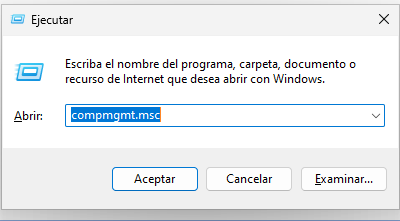
\includegraphics{png/WinRcompmgmt.png}

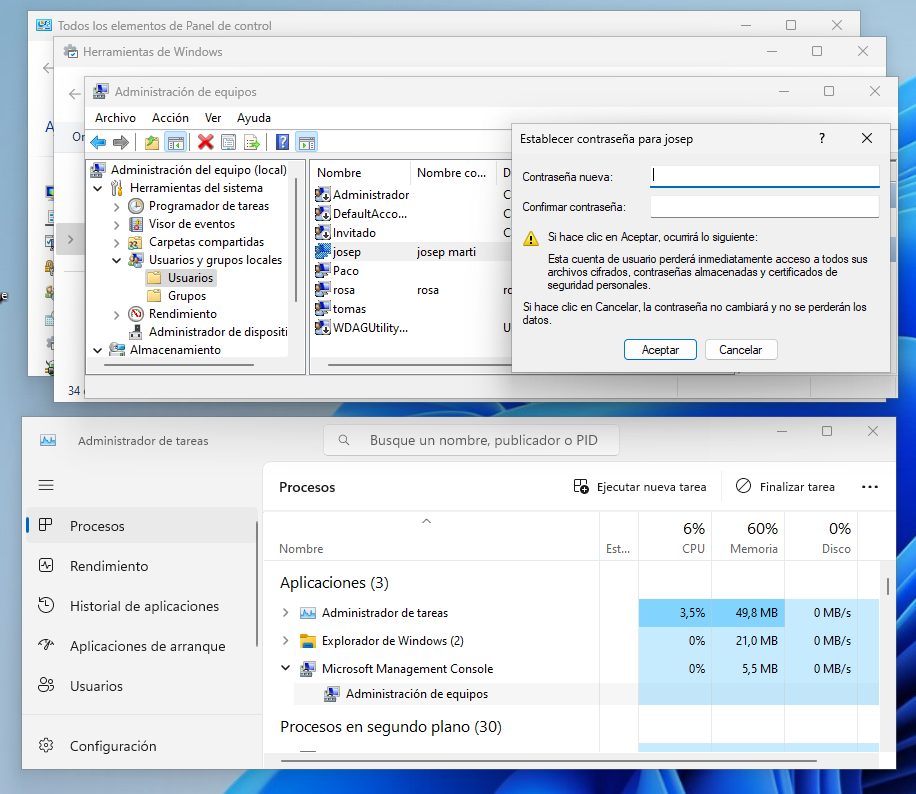
\includegraphics{png/2PaneldeControlHerramientasdeWindowsAdministradordeEquiposUsuariosygruposlocales.png}

\textbf{Avanç}

Les consoles gràfiques de Windows (MSC) Les Microsoft Management Console
(fitxers amb extensió \emph{.msc}) són ferramentes gràfiques per a
tasques d'administració i gestió dels sistemes operatius Windows. Podem
trobar-les al directori d'instal·lació de Windows
\emph{c:\textbackslash windows\textbackslash system32}. Més avant farem
un repàs de totes.

Per accedir directament:

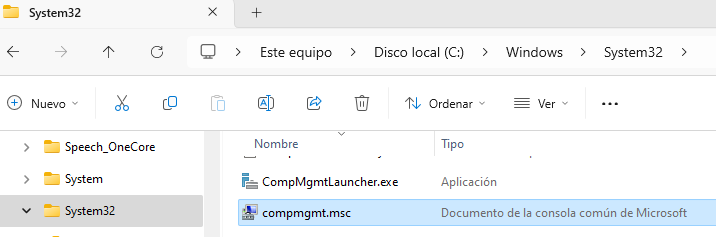
\includegraphics{png/fitxerCompmgmt.png}

\subsection{1.2 ALTRES OPCIONS}\label{altres-opcions}

Des del GUI podem fer algunes gestions amb els comptes d'usuaris.

\subsubsection{1.2.1 Panel de Control. Administrar
cuentas.}\label{panel-de-control.-administrar-cuentas.}

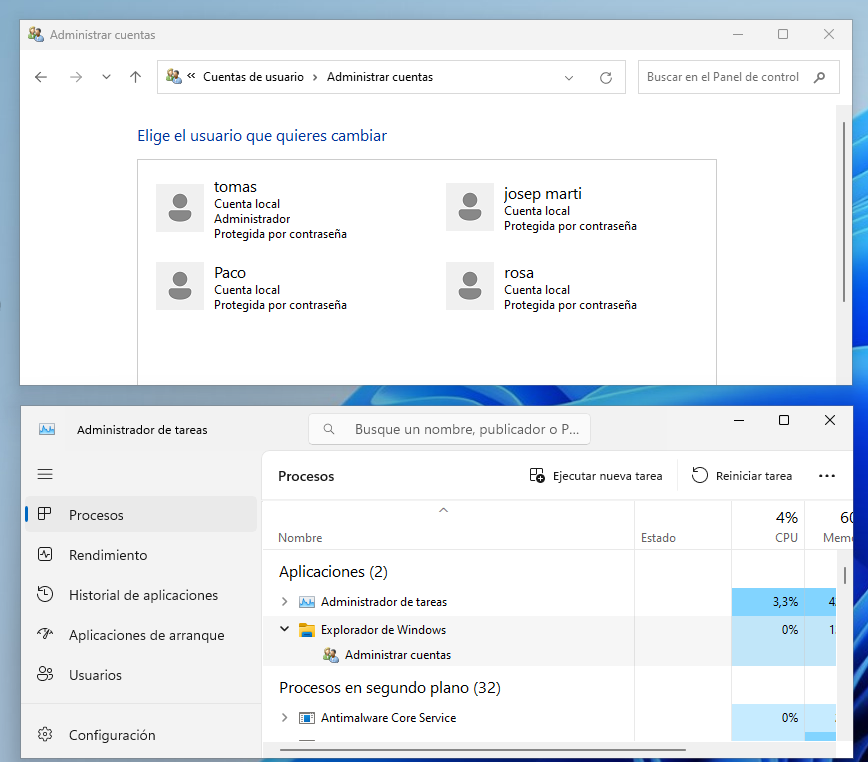
\includegraphics[width=0.8\textwidth,height=\textheight]{png/1PaneldeControlAdministrarCuentas.png}

En esta opció veien que podem canviar el tipus de compte
(Estàndar/Administrador) i poc més.
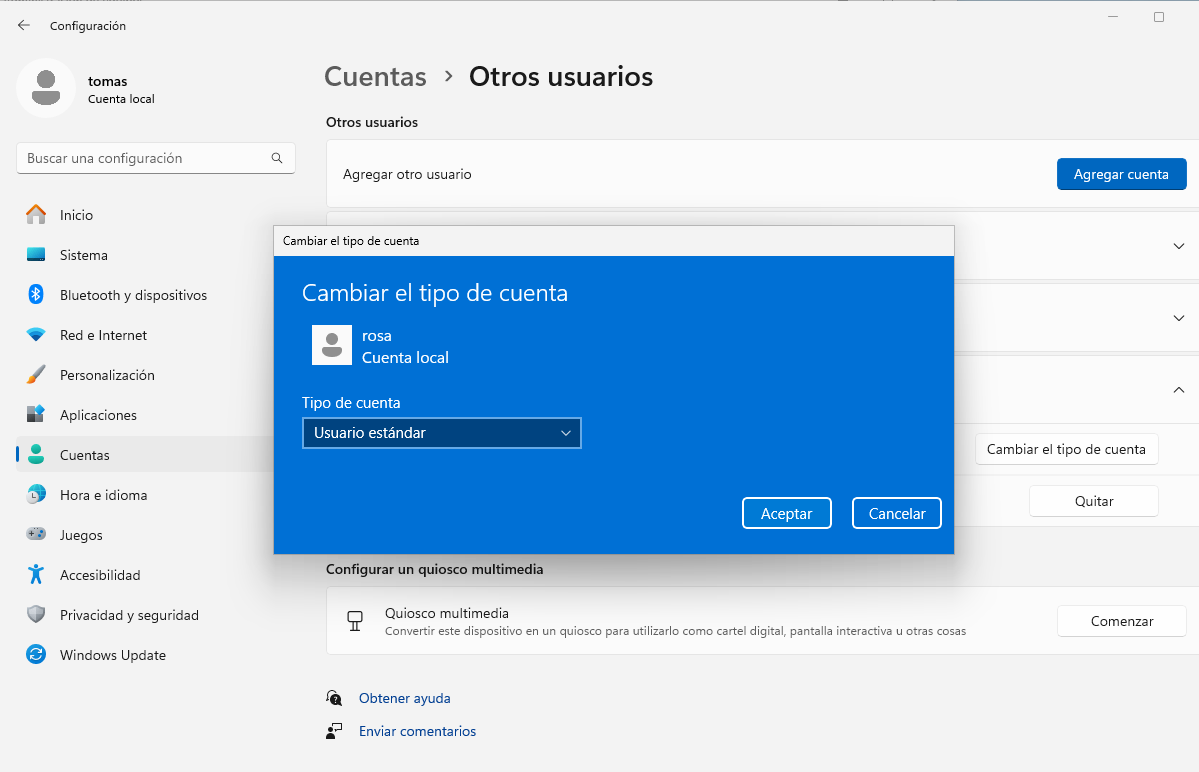
\includegraphics{png/cambiaTipoCuenta.png}

\textbf{Equivalències}

\begin{itemize}
\tightlist
\item
  El tipus per defecte ``Estándard'' equival al grup ``Usuarios''.
\item
  El tipus ``Administradores'' equival al grup d'usuaris
  ``Administradores''
\end{itemize}

\subsubsection{\texorpdfstring{1.2.2 Ferramenta
\emph{netplwiz.exe}}{1.2.2 Ferramenta netplwiz.exe}}\label{ferramenta-netplwiz.exe}

Windows + R i executem \textbf{netplwiz}. Similar als Control Panel
Applets (CPL), components de Panel de Control que en permeten l'accés a
determinades configuracions.

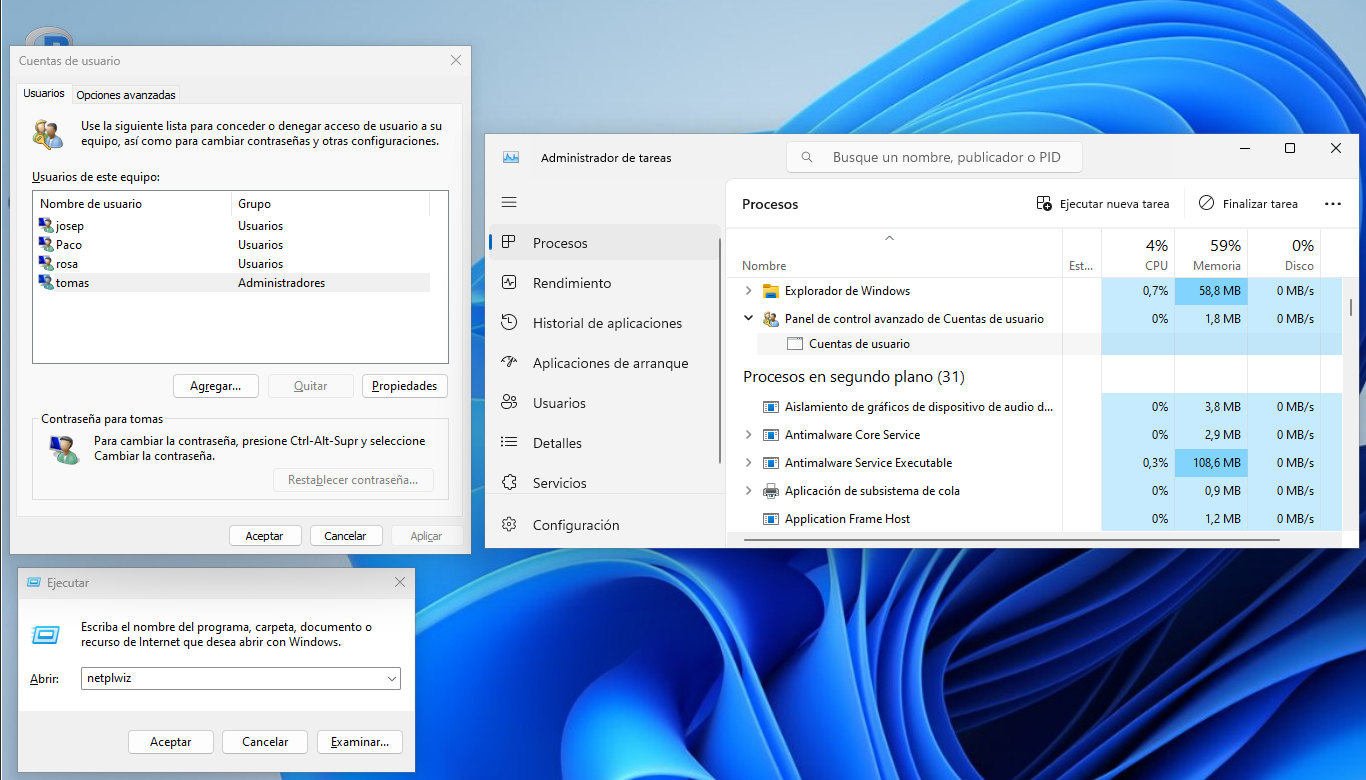
\includegraphics{png/3netplwiz.png}

En esta opció ens mostra els noms de grups d'usuaris als quals pertany
cada usuari. Ens permet afegir a algun grup distint d'Usuarios
(Estándar) i Administradores però no podem crear grups nous.

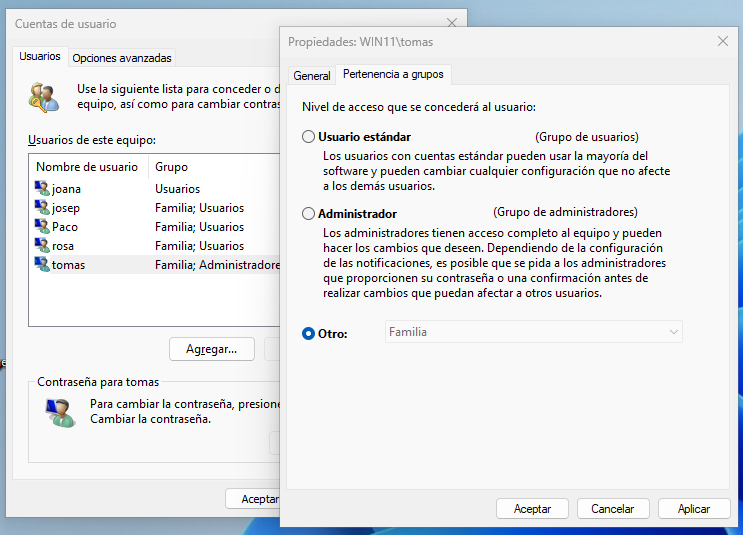
\includegraphics{png/propiedadesNetplwiz.png}

\textbf{Avanç}

Com podem observar a les imatges, cadascuna de les opcions gràfiques en
execució genera un procés distint. A les imatges següents podem observar
les tres alternatives gràfiques obertes al mateix temps i fixar-nos-hi
en les \textbf{tasques (procesos)} que s'hi veuen a
l'\emph{Administrador de Tasques} També veiem com el component de
Windows Consola de Equipos, en executar-se dos vegades, genera dos
processos.

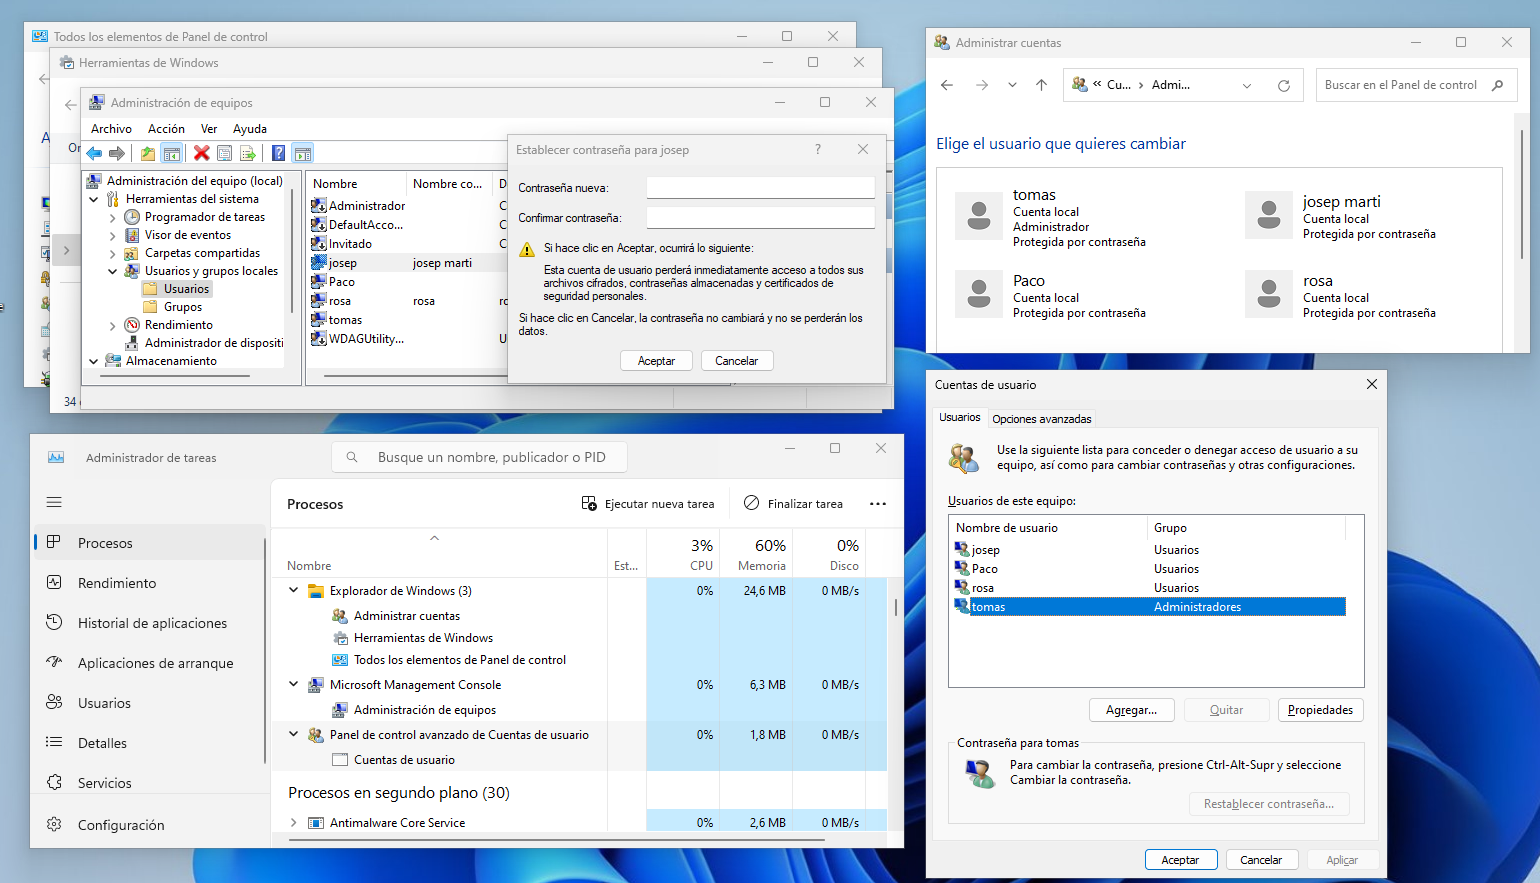
\includegraphics{png/123.png} !{[}{]})png/compmgmtTaskmanager.png)

\section{2 USUARIS I GRUPS}\label{usuaris-i-grups}

\subsection{2.1 Grups per defecte}\label{grups-per-defecte}

La instal·lació de Windows crea uns grups per defecte com veiem a la
imatge següent. Ens centrarem en els dos principals

\begin{itemize}
\item
  El Grup \textbf{Administradores}. Que tindran \textbf{drets} per
  realitzar qualsevol tasca que afecte a la configuració i
  \textbf{permisos} per a modificar carpetes i fitxers.
\item
  El Grup \textbf{Usuarios} No tindran drets per fer cap modificació
  sobre la configuració (per exemple instal·lacions). I només podran fer
  modificacions sobre fitxers i carpetes de la seua propietat.

  Estos grups equivalen al ``tipo de cuenta'',
  ``Administrador/Estándar'' de les opcions del punt 1.2
\end{itemize}

\subsection{2.2 Nous grups d'usuari}\label{nous-grups-dusuari}

A banda d'estos dos grups básics, existeixen altres que crea també el
sistema per al seu propi funcionament, però a nosaltres pot
interessar-nos crear altres grups d'usuaris amb la finalitat d'establir
quines persones poden fer determinades coses i quines altres no sobre
les carpetes i fitxers o sobre el software de la màquina.

A l'exemple que veiem hem creat un grup amb el nom ``Familia''.

\begin{quote}
Avanç: Un \textbf{permís} és una autorització sobre que se li dóna a un
usuari (o grup) per a poder:

\begin{enumerate}
\def\labelenumi{\arabic{enumi}.}
\tightlist
\item
  Llegir o
\item
  Escriure o
\item
  Canviar els permisos (1 i 2) o el \emph{propietari}
\end{enumerate}

unes carpetes o fitxers

El \textbf{propietari} és, per defecte, l'usuari que ha creat la carpeta
o fitxer.

( Ho abordarem més avant )
\end{quote}

El que hem de tenir en compte és que, si bé per defecte un usuari és
\emph{administrador} o \emph{estándard} de forma exclusiva, podem crear
nous grups i incloure-hi els usuaris que vullguem.

Fixem-nos a la imatge següent. Observem que hem creat un grup
``Familia'' al qual hem afegit un usuari que pertany al grup
``Administradores'' ( Tomas) i també un usuari estandard del grup
``Usuarios''

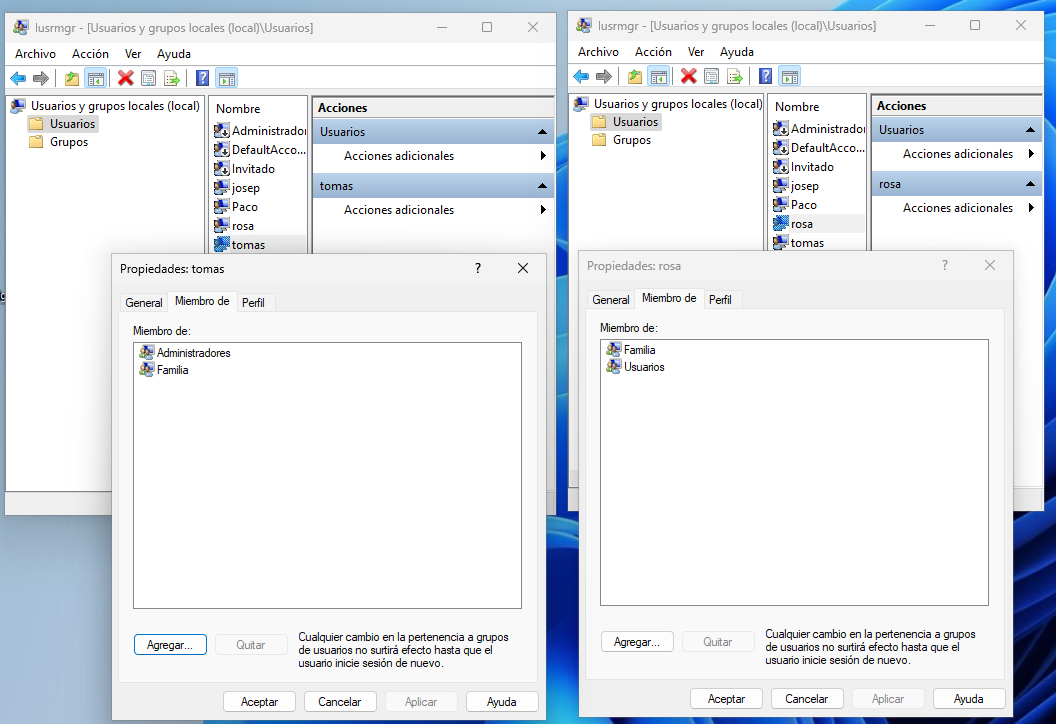
\includegraphics[width=0.8\textwidth,height=\textheight]{png/mesdungrup.png}

\subsection{2.3 Acumulació de permisos de lectura, escriptura o
canvi}\label{acumulaciuxf3-de-permisos-de-lectura-escriptura-o-canvi}

Per tant, un mateix usuari pot pertànyer a més d'un grup. En estos
casos, els permisos de cadascun dels grups als quals pertany se sumen.

\begin{quote}
A la següent secció estudiarem el permisos amb més detall.
\end{quote}

\section{3. VISIÓ DES DE L'INTERFACE DE
COMANDAMENTS}\label{visiuxf3-des-de-linterface-de-comandaments}

Encara que en Windows11 serà més habitual treballar en l'entorn gràfic
hem de tenir sempre present que disposem de dos shells o interface de
comandaments:

\begin{itemize}
\tightlist
\item
  La consola de comandaments o cmd
\item
  Powershell
\end{itemize}

En una unitat següent s'estudiarà com crear modificar comptes des
d'estos entorns CLI. Ara, fem este avanç només per comprovar que els
usuaris estan creats però el seu perfil ( carpetes encara no ).

\subsection{3.1 Des de la consola CMD:}\label{des-de-la-consola-cmd}

Pulsem \emph{Win-R : cmd} i comprovem amb

\begin{Shaded}
\begin{Highlighting}[]
\NormalTok{net users}
\end{Highlighting}
\end{Shaded}

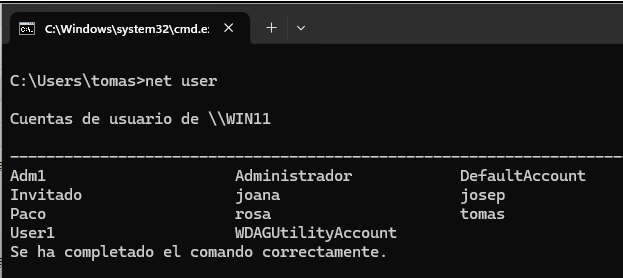
\includegraphics{png/netUser.png}

\begin{Shaded}
\begin{Highlighting}[]
\NormalTok{net localgroup}
\end{Highlighting}
\end{Shaded}

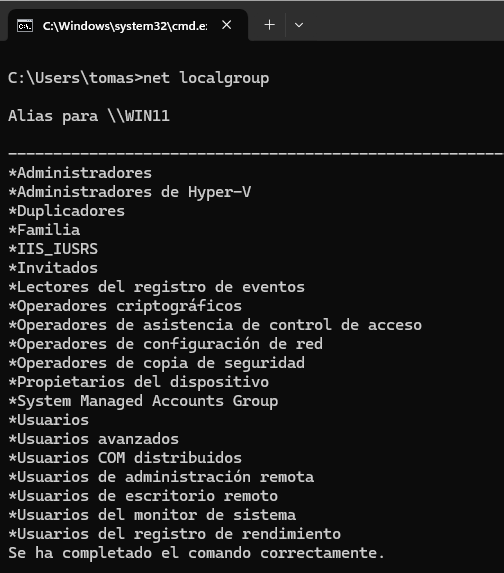
\includegraphics{png/netLocalGroup.png}

\subsection{3.2 Des de Powershell}\label{des-de-powershell}

Puelsem \emph{Win-R: powershell} i comprovem amb

\begin{Shaded}
\begin{Highlighting}[]
\NormalTok{get{-}LocalUser}
\end{Highlighting}
\end{Shaded}

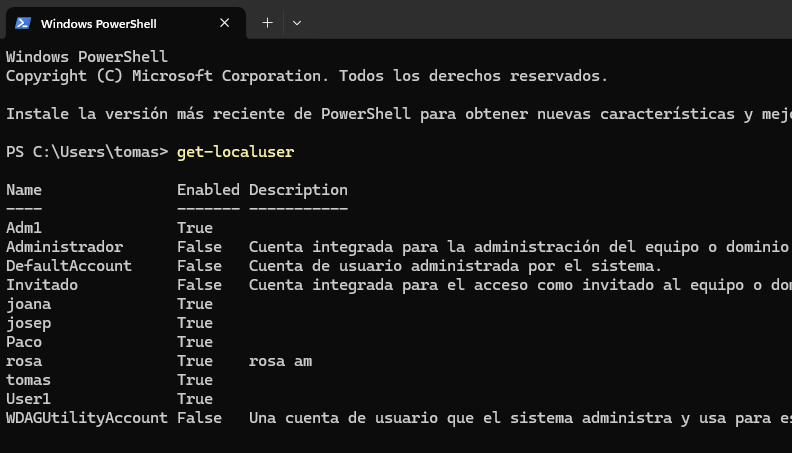
\includegraphics{png/get-LocalUser.png}

\begin{Shaded}
\begin{Highlighting}[]
\NormalTok{get{-}LocalGroup}
\end{Highlighting}
\end{Shaded}

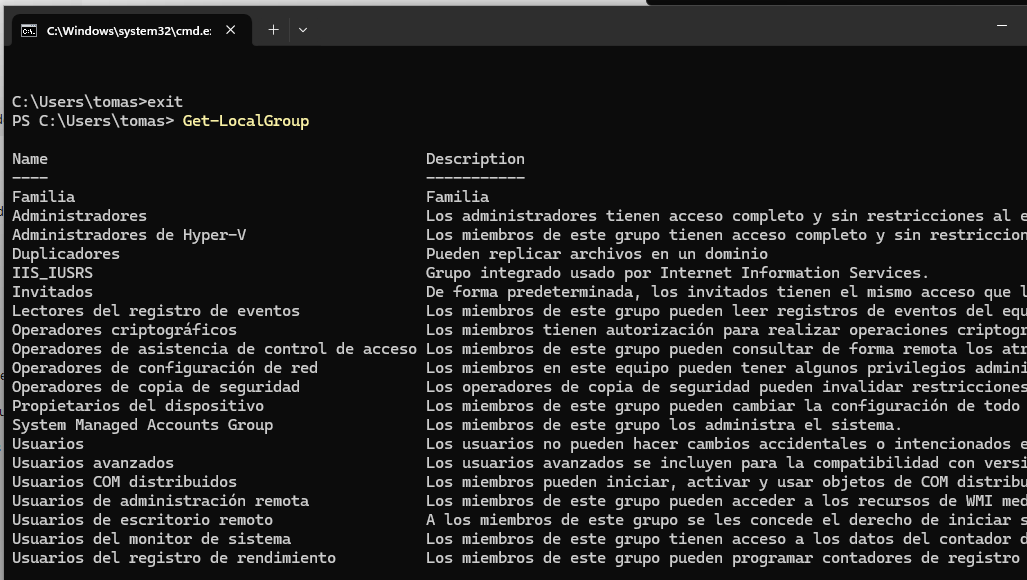
\includegraphics{png/get-LocalGroup.png}

\section{5 VISIÓ AL REGISTRE del
SISTEMA}\label{visiuxf3-al-registre-del-sistema}

Observem com es registra al Registre del sistema els perfils (profiles)
de cada usuari. \textbf{Avanç} El Registre del sistema
(\emph{C:\textbackslash WINDOWS\textbackslash regedit.exe}) és un
component essencial de tots el sistemes Windows. Formalment és una base
de dades jeràrquica que emmagatzema configuracions i opcions del sistema
operatiu i les aplicacions.

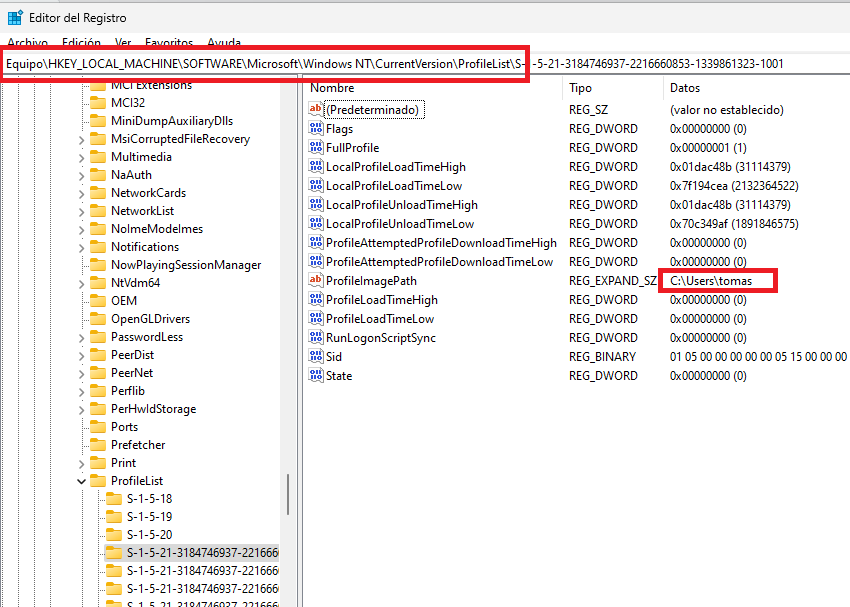
\includegraphics{png/regedit.png}

\section{4 PERFIL DE L'USUARI}\label{perfil-de-lusuari}

El perfil comprén tots els directoris ( ``Els meus Documents,
Descàrregues\ldots{}'') i altres característiques que són exlusives de
cada usuari o comuns.

Veiem les carpetes: 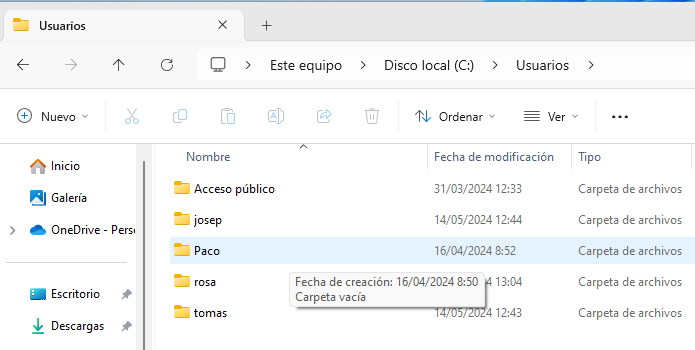
\includegraphics{png/users.png}

\subsection{4.1 Creació del perfil}\label{creaciuxf3-del-perfil}

Segurament si hem creat un usuari nou, haurem comprovat en l'anterior
punt que l'usuari acabat de crear:

\begin{itemize}
\tightlist
\item
  Apareix al GUI. Consola gràfica 8 compmgmt.msc ) i les altres opcions.
\item
  Apareix al CLI. \emph{net user} i \emph{get-localuser}
\item
  No apareix al registre del sistema la entrada a \emph{ProfileList}
\item
  No apareixen les carpetes de perfil personal a
  \emph{C:\textbackslash usuarios}
\end{itemize}

\begin{quote}
Quan es crea el perfil de l'usuari? El perfil dels usuaris (
c:\textbackslash users\textbar usuari\textbackslash\ldots es crea quan,
una vegad creat, iniciem per primera vegada sessió amb ell. Notarem que
el primer inci de sessió es fa molt lent, sobretot si no hem desactivat
Cortana Com a nota podem avançar que en Linux veurem que ocorre el
mateix.
\end{quote}

Una vegada creat el perfil, podem entrar dins de la carpeta del nostre
usuari i observar tres subcarpetes:

\begin{itemize}
\tightlist
\item
  Default
\item
  Públic
\item
  Carpeta específica de cada usuari
\end{itemize}

Cadascuna té una funció que veiem tot seguit.

\subsection{4.1 Default}\label{default}

La carpeta \textbf{Default} és una plantilla per a la creació de nous
perfils d'usuari. Conté configuracions i arxius predeterminats que es
copien a qualsevol nou compte d'usuari quan es crea. Ací es troben:

\begin{itemize}
\tightlist
\item
  \textbf{Configuracions del compte}: Preferències i configuracions
  d'aplicacions predeterminades.
\item
  \textbf{Carpetes d'usuari predeterminades}: Documents, Imatges,
  Música, Vídeos, Escriptori, Descàrregues, etc.
\item
  \textbf{Arxius de configuració}: Arxius de personalització de l'entorn
  d'usuari, com el fons d'escriptori, icones, accessos directes, etc.
\end{itemize}

Els nous usuaris de l'ordinador hereten estos arxius i configuracions la
primera vegada que inicien sessió.

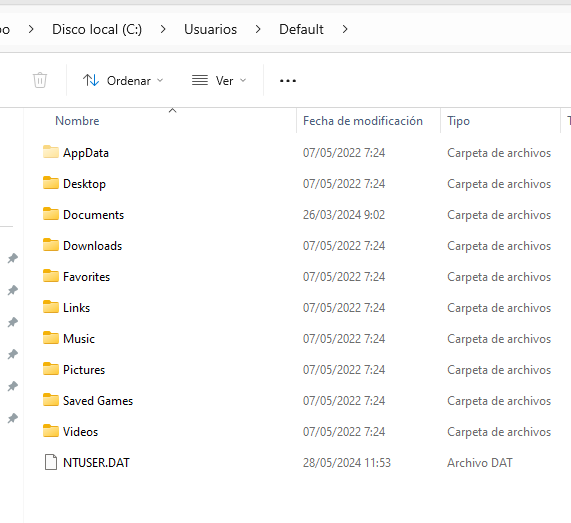
\includegraphics{png/CarpetesDefault.png}

\subsection{4.2 Públic}\label{puxfablic}

La carpeta \textbf{Públic}. Carpeta compartida accessible per tots els
usuaris de l'equip per compartir arxius sense cap restricció.

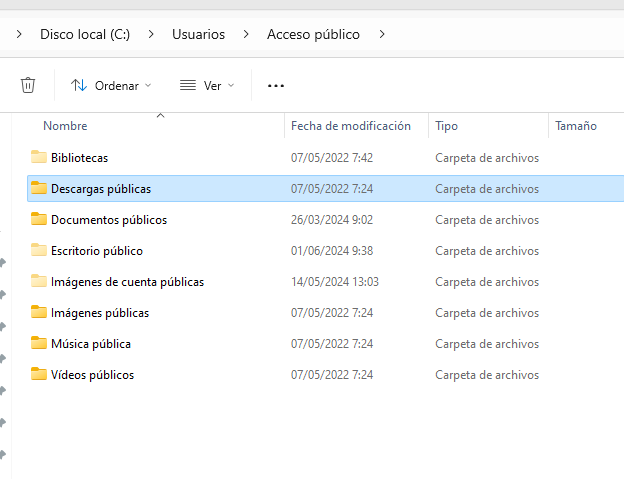
\includegraphics{png/CarpetesPublico.png}

\subsection{4.3 Carpeta de l'Usuari
Específic}\label{carpeta-de-lusuari-especuxedfic}

Cada usuari té la seva pròpia carpeta, que emmagatzema els seus arxius
personals i configuracions específiques. Esta carpeta inclou:

\begin{itemize}
\tightlist
\item
  \textbf{Carpetes personals}: Documents, Imatges, Música, Vídeos,
  Escriptori, Descàrregues.
\item
  \textbf{Configuracions d'usuari}: Configuracions específiques de
  l'usuari que afectaran a com pot usar el SO i aplicacions software.
\item
  \textbf{Arxius i configuracions personals}: Qualsevol arxiu que
  l'usuari guarde a seues carpetes personals i també les configuracions
  personalitzades.
\end{itemize}

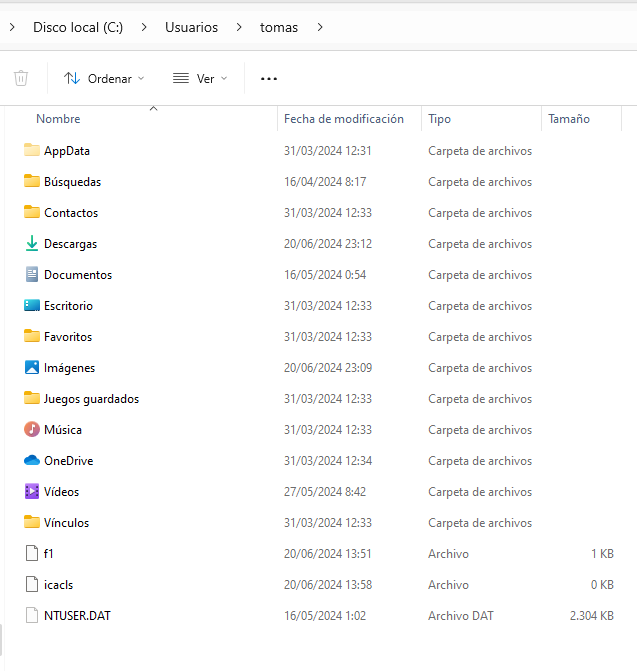
\includegraphics{png/CarpetesPerfil.png}

\begin{quote}
Només podrem entrar a carpeta d'altres usuaris si som Administrador. Es
proposa més avant una activitat per comprovar-ho.
\end{quote}

\section{5 Activitats}\label{activitats}

\subsection{Activitat 1}\label{activitat-1}

\begin{enumerate}
\def\labelenumi{\arabic{enumi}.}
\tightlist
\item
  Des de la Consola gràfica, crea un usuari que pertanya al grup
  Administradores i un altre que siga no, només al grup Usuarios amb els
  noms respectius:
\end{enumerate}

\begin{itemize}
\tightlist
\item
  Adm1
\item
  User1
\end{itemize}

\begin{enumerate}
\def\labelenumi{\arabic{enumi}.}
\setcounter{enumi}{1}
\item
  Assegura't que l'usuari haja de canviar la contrassenya la primera
  vegada d'iniciar sessió en els dos usuaris.
\item
  Inicia sessió, amb l'usuari \emph{Adm1}. 3.1 Crea un fitxer
  \emph{Doc1.txt} a la carpeta personal de Adm1
  C:\textbackslash users\textbackslash Adm1\textbackslash Documentos 3.2
  Crea un nou fitxer \emph{EnPublic.txt} i guarda'l a la carpeta
  C:\textbackslash Public\textbackslash Documents 3.3 Crea una carpeta
  de
  C:\textbackslash Default\textbackslash Documents\textbackslash Defecte
  3.4 Dins d'esta, crea un fitxer \emph{def1.txt} 3.4 Observa els
  continguts de les carpetes C:\textbackslash Users\textbackslash Adm1 i
  C:\textbackslash Users\textbackslash User1
\item
  Inicia sessió amb \emph{User1}. Ara comprovarem l'efecte dels canvis
  fets adés en este usuari nou.

  4.1 Entra al perfil de User1
  C:\textbackslash users\textbackslash User1 4.2 Comprova si apareix la
  carpeta \emph{Defecte} i el seu contingut. 4.3 Intenta entrar a Public
  i mira qué tens
\end{enumerate}

\end{document}
